\documentclass[a4paper]{article}
\setlength{\evensidemargin}{-4mm}    % This changes margin values
\setlength{\oddsidemargin}{1cm}
\setlength{\textwidth}{6.0in}
\setlength{\textheight}{8.2in}
\setlength{\headsep}{0.4in}
\setlength{\parindent}{0pt}            

\usepackage[pdftex]{graphics}
\usepackage{multirow}
\usepackage{fancyhdr}           % This put a frame in the title      
\pagestyle{fancy}               % of every chapter.  They work 
\usepackage[Lenny]{fncychap}    % by including the file: 
%\usepackage[dvips]{graphicx}    % 'fncychap.sty'
%\usepackage[dvips]{color,graphicx} % 
%\usepackage{array}                     
\usepackage[activeacute,english]{babel}
%\usepackage{graphics}
\usepackage{float}
\usepackage{latexsym}
\usepackage{amsmath}
\usepackage[small]{caption2}   % Font size for captions  
%\usepackage{feynmf}%%%{feynmp}  % To draw Feynman diagrams
%\unitlength = 1mm
\usepackage{graphicx}
\usepackage{amssymb}
\usepackage{amsmath,amsfonts,amsthm,amssymb}
\usepackage{epstopdf}
\usepackage{setspace} 
\usepackage{footmisc}	
\usepackage{enumitem}
\usepackage{mathtools}
\usepackage{eqnarray,amsmath}
\usepackage{color}


\setlength{\topmargin}{-10mm}
\setlength{\textwidth}{7in}
\setlength{\oddsidemargin}{-8mm}
\setlength{\textheight}{9in}
\setlength{\footskip}{1in}	

\title{Generator for Various Channels of $\gamma d\rightarrow K^+X$}
\author{Tongtong Cao}
\date{\today}

\begin{document}
\fontsize{12}{15}
\selectfont
\maketitle
\section{Introduction}
The generator involves 9 channels of $\gamma d\rightarrow K^+X$, including 5 channels for $\Lambda$ production, 2 channels for $\Sigma$ production, 1 channel for $\Sigma^{*0}$ production and 1 channel for $\Sigma^{*-}$ production. For all channels, beam and target are the same. Energy of the photon beam is randomly generated by optional models. Fermi momentum of nucleons bounded in the target deterium is randomly generated by the Paris model using the reject-accept method. In general, re-scattering channels are processed by two steps, while quasi-free channels are process by one step. Besides, there are decay processings.  For each channel excluding $\Sigma^{*0}$ and $\Sigma^{*-}$ production channels, corresponding unpolarized and/or polarized differential cross section (DCS) are implemented to select events of channels, i.e. to set weights for channels, in the first and/or second steps. The generater is multi-funcitonal and flexible. Some options are offered to users for various requirements of analysis.

\section{Scheme of Generator}
Figure~\ref{scheme} shows the general processing of the generator. Initially for an event, the photon beam energy is generated and random number (RN) 1 and 2 are used to generate the fermi momentum so that Lorentz vectors of the beam, the first and the second targets are fixed. The first target is one nucleon in the deterium, which is off-shell, and the second target is the other nucleon, which is on-shell. Next, a RN is used to randomly select a channel for the event. After the event enters the selected channel, the phase base calculation for the first step is implemented so that Lorentz vectors of 2 produced particle are calculated, and then unpolarized (or polarized) DCS is calculated to determine if the event is accepted or rejected by comparing it to RN3 for unpolarized DCS (or RN4C for circularly polarized DCS or RN4L for linearly polarized DCS). If the event is accpted, it enters the second step. For the second step, the beam is one of particles produced by the first step. Like the fist step, the phase base calculation is firstly implemented so that Lorentz vectors of 2 produced particle are calculated, and then unpolarized differental cross section is calculated to determine if the event is accepted or rejected  by comparing it to RN5. 

\begin{figure}[H]
   \begin{center}
   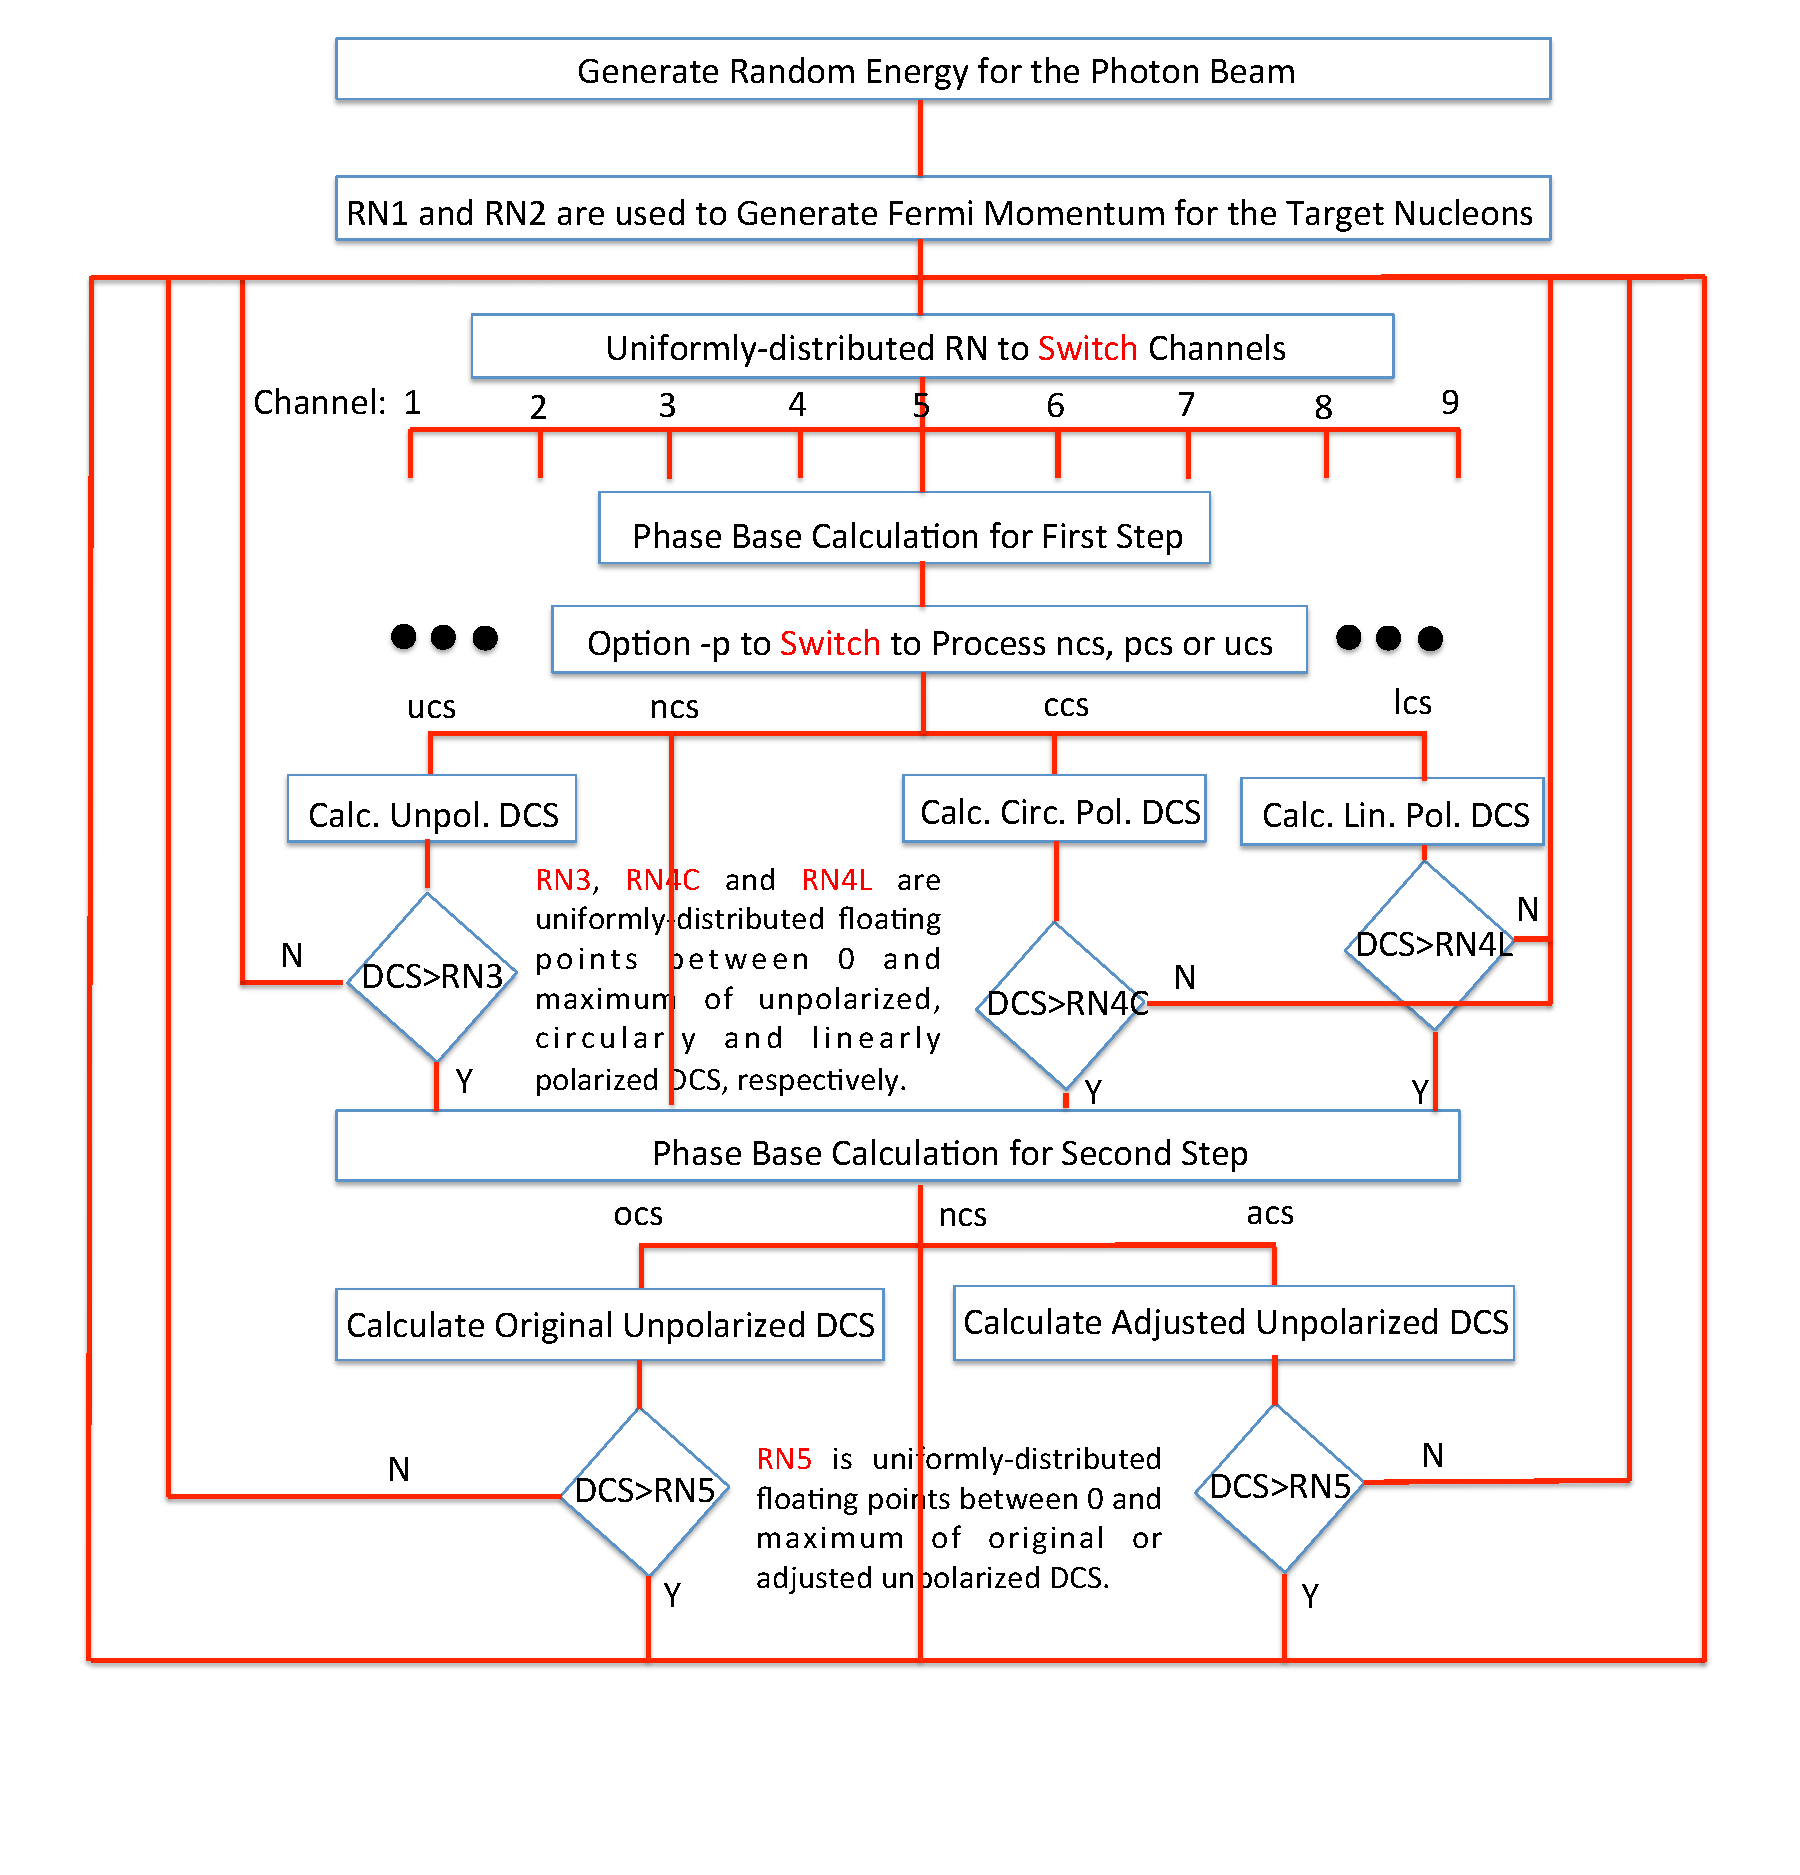
\includegraphics[width=6.8in,height=7.2in]{flow-chart.pdf} 
   \caption[]{Scheme of Generator}      \label{scheme}
   \end{center}
\end{figure}

Due to exceptional situations of each channel, the real processing is different between channels. The detailed processing for each channel is discussed in the following.

\begin{enumerate}
\item $\pi^0$ mediated re-scattering of $\gamma d\rightarrow K^+\Lambda n$
  \begin{itemize}
  \item Step 1: $\gamma n\rightarrow \pi^0 n$
  \item Step 2: $\pi^0 p\rightarrow \Lambda K^+$
  \item Step decay: $\Lambda\rightarrow p \pi^-$
  \end{itemize}

\item $K^+ n$ re-scattering of $\gamma d\rightarrow K^+\Lambda n$
  \begin{itemize}
  \item Step 1: $\gamma p\rightarrow  \Lambda K^+$
  \item Step 2: $K^+ n\rightarrow K^+ n$
  \item Step decay: $\Lambda\rightarrow p \pi^-$
  \end{itemize}

Since kinematics of proton are required to calculate polarized DCS for the first step, the third step is implemented.

\item $\Lambda n$ re-scattering of $\gamma d\rightarrow K^+\Lambda n$
  \begin{itemize}
  \item Step 1: $\gamma p\rightarrow \Lambda K^+$ 
  \item Step 2: $\Lambda n\rightarrow \Lambda n$
  \item Step decay: $\Lambda\rightarrow p \pi^-$
  \end{itemize}

\item $\Sigma n$ re-scattering of $\gamma d\rightarrow K^+\Sigma n$
  \begin{itemize}
  \item Step 1: $\gamma p\rightarrow \Sigma K^+ $
  \item Step 2: $\Sigma n\rightarrow \Sigma n$
  \end{itemize}

\item $\pi^+$ mediated re-scattering of $\gamma d\rightarrow K^+\Lambda n$
  \begin{itemize}
  \item Step 1: $\gamma p\rightarrow \pi^+ n$
  \item Step 2: $\pi^+ n\rightarrow \Lambda K^+$
  \item Step decay: $\Lambda\rightarrow p \pi^-$
  \end{itemize}

\item Quasi-free of $\gamma d\rightarrow K^+\Sigma^{*0} n$
  \begin{itemize}
  \item Step 1: $\gamma p\rightarrow \Sigma^{*0} K^+$
  \item Step decay: $\Sigma^{*0}\rightarrow \Lambda\pi^0$
  \end{itemize}

\item Quasi-free of $\gamma d\rightarrow K^+\Sigma^{*-} p$
  \begin{itemize}
  \item Step 1: $\gamma n\rightarrow \Sigma^{*-} K^+$
  \item Step decay: $\Sigma^{*-}\rightarrow \Lambda\pi^-$
  \end{itemize}

\item Quasi-free of $\gamma d\rightarrow K^+\Lambda n$
 \begin{itemize}
  \item Step 1: $\gamma p\rightarrow  \Lambda K^+$
  \item Step decay: $\Lambda\rightarrow p \pi^-$
  \end{itemize}

\item Quasi-free of $\gamma d\rightarrow K^+\Sigma n$
  \begin{itemize}
  \item Step 1: $\gamma p\rightarrow  \Sigma K^+$
  \end{itemize}

\end{enumerate}


\section{Discussion about DCS and RN}
For 1 step of a channel, unpolarized DCS is calculated based on kinematcis and the corresponding unpolarized DCS table, and polarized DCS is calculated based on kinematcis, the corresponding unpolarized DCS and polarization observable tables. RN3 and RN5 are uniformly-distributed floating points between 0 and maximum of the corresponding unpolarized DCS, and RN4C and RN4L is uniformly-distributed floating points between 0 and maximum of the corresponding polarized DCS. If unpolarized (or polarized) DCS is larger than RN, the event is accpeted, otherwise it is rejected.

For calculating unpolarized or polarized DCS, unpolarized DCS and polarization observable tables are made through collecting information from various databases.

\begin{enumerate}
\item Unpolarized DCS tables for the first step of channels 1, 2, 3, 4, 5, 8 and 9
 \begin{itemize}
  \item Unpolarized DCS table for $\gamma n\rightarrow\pi^0 n$: $W$: [1.075, 2] GeV; $\theta_{cm}$: [0, 180]; Maximum of unpolarized DCS: 30.9
  \item Unpolarized DCS table for $\gamma p\rightarrow K^+\Lambda$: $W$: [1.61, 2.2] GeV; $\theta_{cm}$: [0, 180]; Maximum of unpolarized DCS: 0.355
  \item Unpolarized DCS table for $\gamma p\rightarrow K^+\Sigma$: $W$: [1.687, 2.2] GeV; $\theta_{cm}$: [0, 180]; Maximum of unpolarized DCS: 0.265
  \item Unpolarized DCS table for $\gamma p\rightarrow\pi^+ n$: $W$: [1.08, 2] GeV; $\theta_{cm}$: [0, 180]; Maximum of unpolarized DCS: 24.8
  \end{itemize}

\item Linear polarization observable $\Sigma$ tables to calcualte polarized DCS with combination of unpolarized DCS for the first step of channels 1 and 5; Table is built based on the Said database.
 \begin{itemize}
  \item $\Sigma$ table for $\gamma n\rightarrow\pi^0 n$: $E$: [0.9, 2.6] GeV; $\theta_{cm}$: [0, 180]; Maxium of polarized DCS: 24 determined by the distribution in Fig.~\ref{pdcs-value-pi0}

\begin{figure}[H]
   \begin{center}
   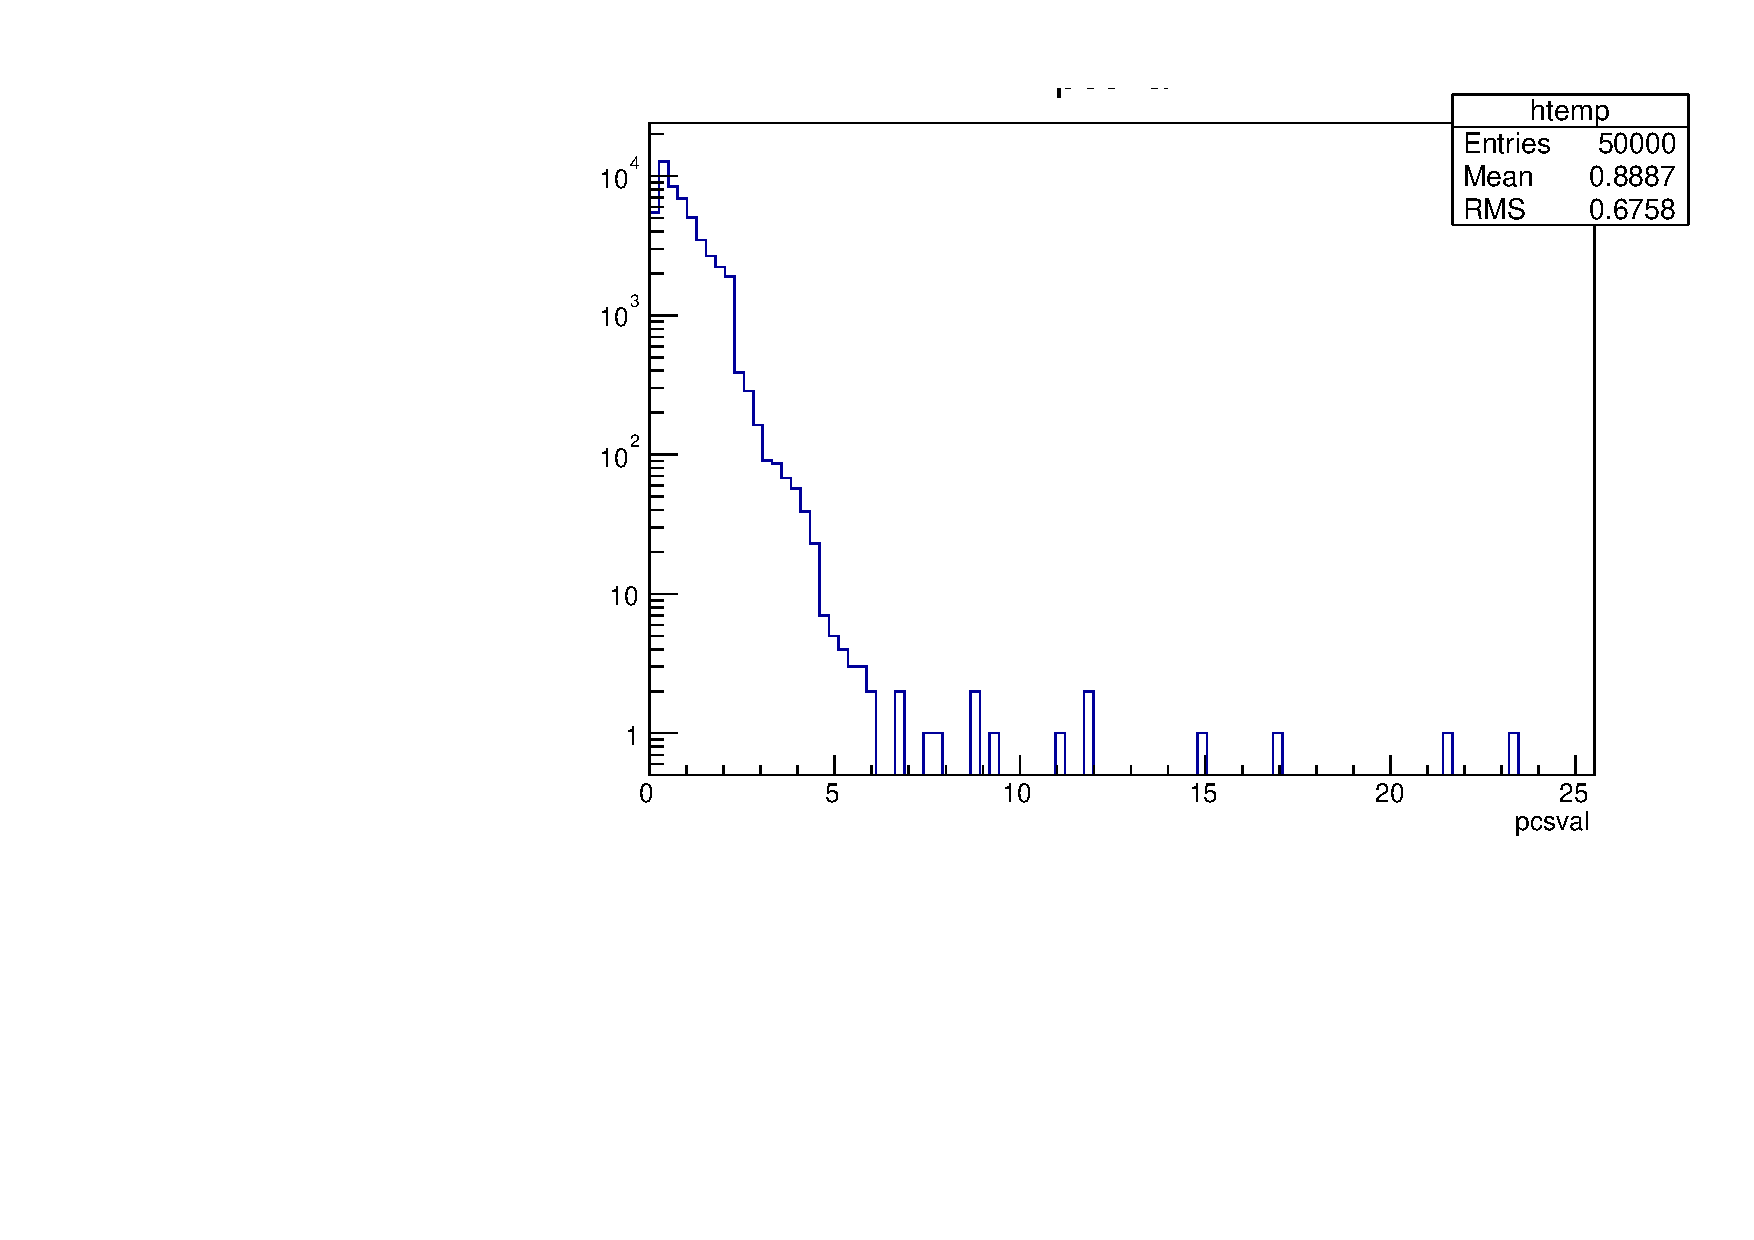
\includegraphics[width=6in,height=3in]{pdcs-value-pi0.pdf} 
   \caption[]{Distribution of polarized DCS for $\gamma n\rightarrow\pi^0 n$}      \label{pdcs-value-pi0}
   \end{center}
\end{figure}

  \item $\Sigma$ table for $\gamma p\rightarrow\pi^+ n$: $E$: [0.9, 2.6] GeV; $\theta_{cm}$: [0, 180];
Maxium of polarized DCS: 23 determined by the distribution in Fig.~\ref{pdcs-value-pi+}

\begin{figure}[H]
   \begin{center}
   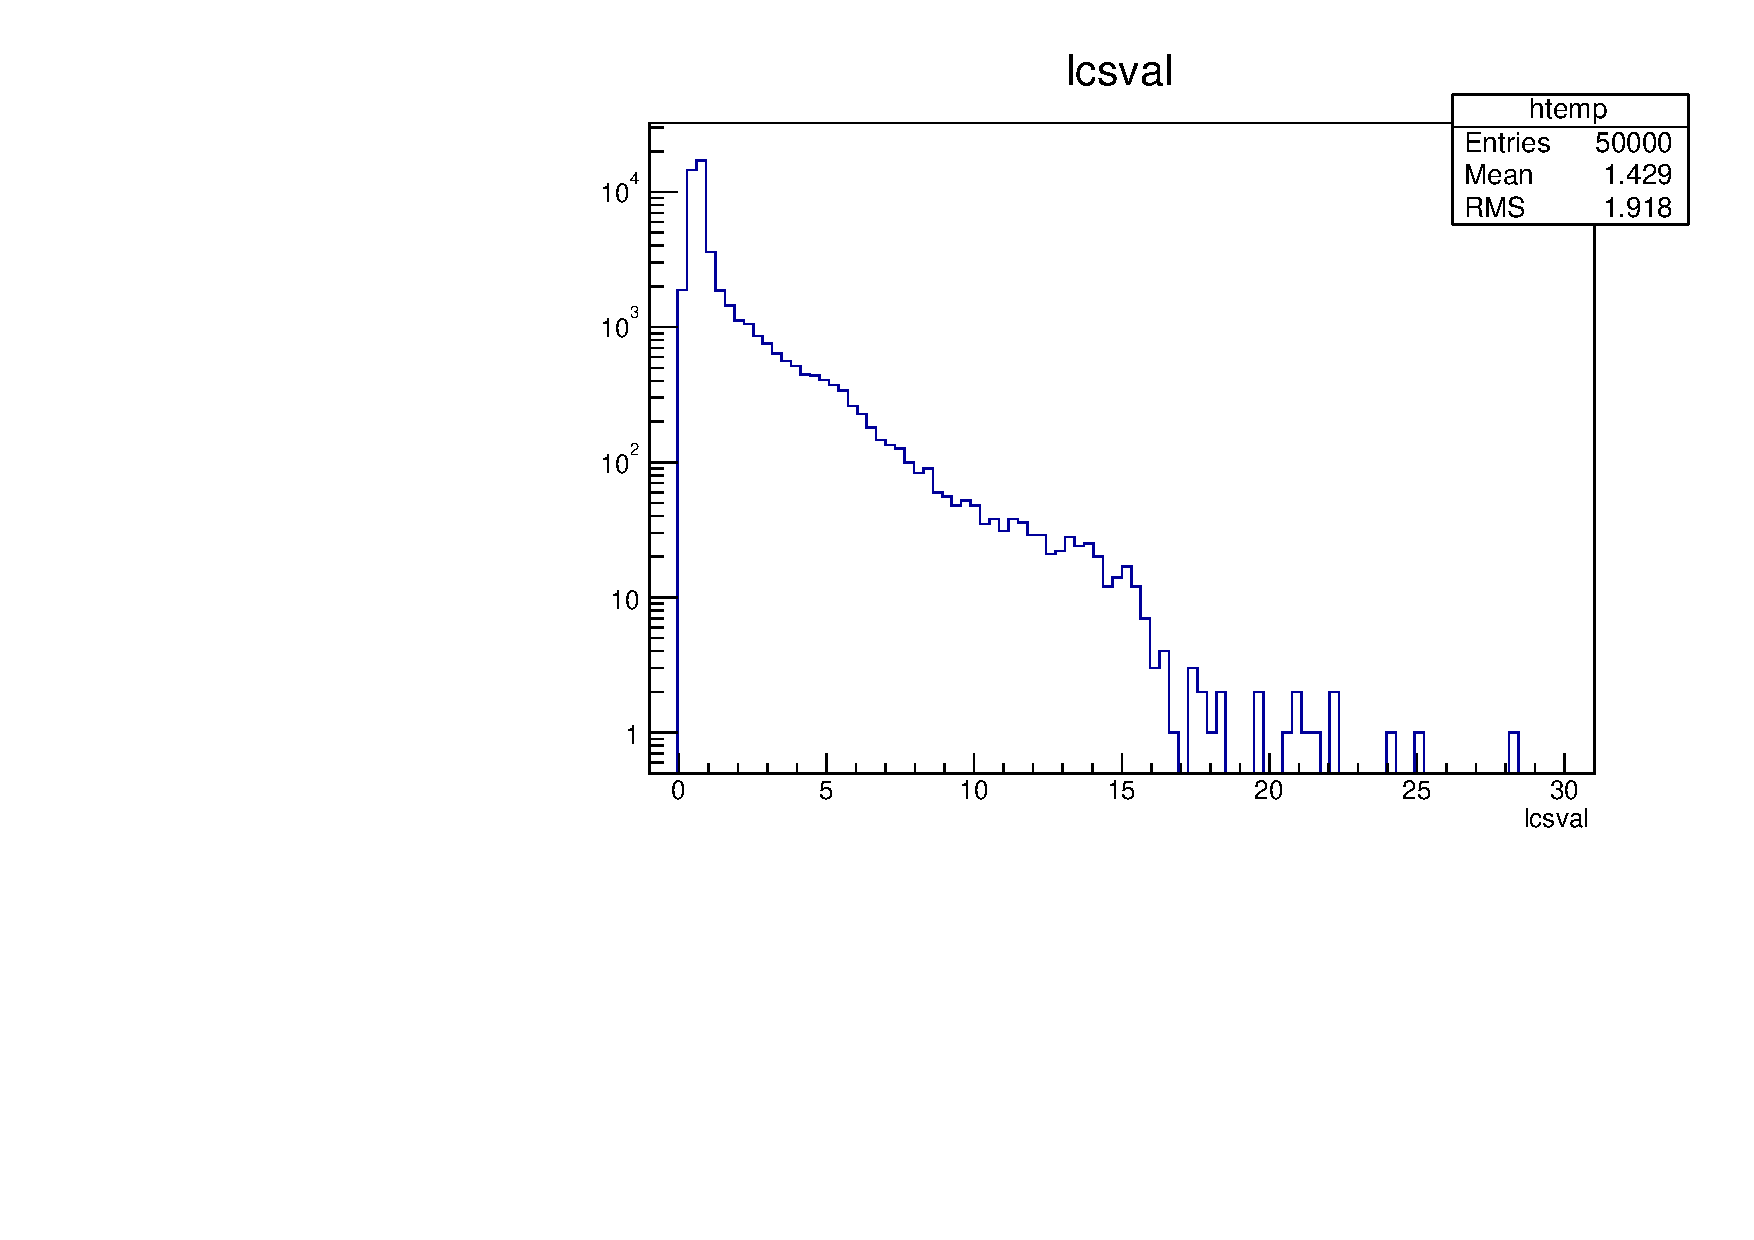
\includegraphics[width=6in,height=3in]{pdcs-value-pi+.pdf} 
   \caption[]{Distribution of polarized DCS for $\gamma p\rightarrow\pi^+ n$}      \label{pdcs-value-pi+}
   \end{center}
\end{figure}

  \end{itemize}


\item Circular polarization observable $C_x$, $C_z$ and $P_y$ table to calculate circularly polarized DCS with combination of unpolarizaed DCS for the first step of channel 2. Table is from results of the CLAS g13a experiment by T. Cao et al.
 \begin{itemize}
  \item $C_x$, $C_z$ and $P_y$ table for $\gamma p\rightarrow K^+\Lambda$: $E$: [0.9, 2.6] GeV; $\cos\theta_{cm}$: [-1, 1]; Maxium of circularly polarized DCS: 0.58 determined by the distribution in Fig.~\ref{pdcs-value-KN}

\begin{figure}[H]
   \begin{center}
   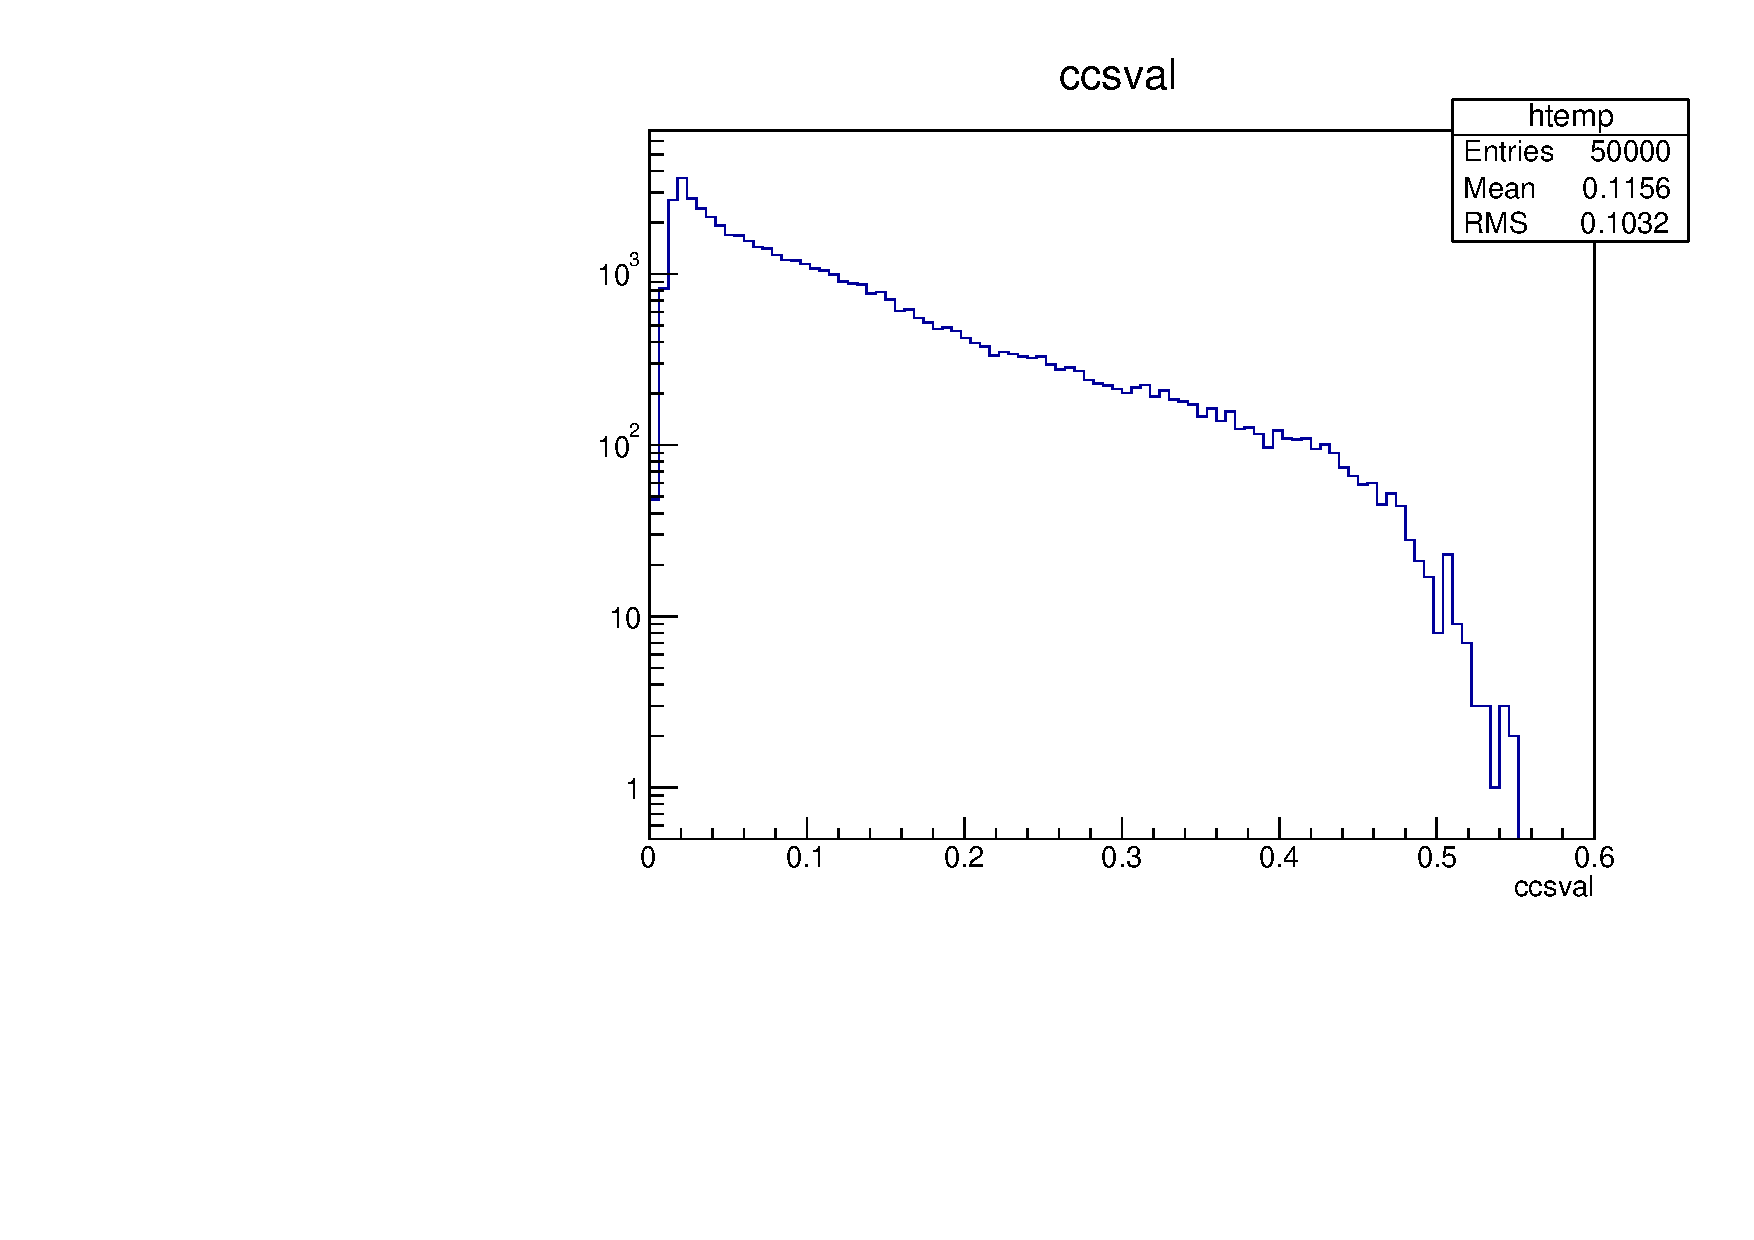
\includegraphics[width=6in,height=3in]{pdcs-value-KN.pdf} 
   \caption[]{Distribution of circularly polarized DCS for $\gamma p\rightarrow K^+\Lambda$}      \label{pdcs-value-KN}
   \end{center}
\end{figure}

  \end{itemize}

\item Linear polarization observable $\Sigma$, $T$, $O_x$, $O_z$ and $P_y$ table to calculate linearly polarized DCS with combination of unpolarizaed DCS for the first step of channel 2. Table is from results of the CLAS g8 experiment by C. A. Paterson et al.
 \begin{itemize}
  \item $\Sigma$, $T$, $O_x$, $O_z$ and $P_y$ table for $\gamma p\rightarrow K^+\Lambda$: $W$: [1.72, 2.18] GeV; $\cos\theta_{cm}$: [-65, 0.75]; Maxium of linearly polarized DCS: 0.80 determined by the distribution in Fig.~\ref{ldcs-value-KN}

\begin{figure}[H]
   \begin{center}
   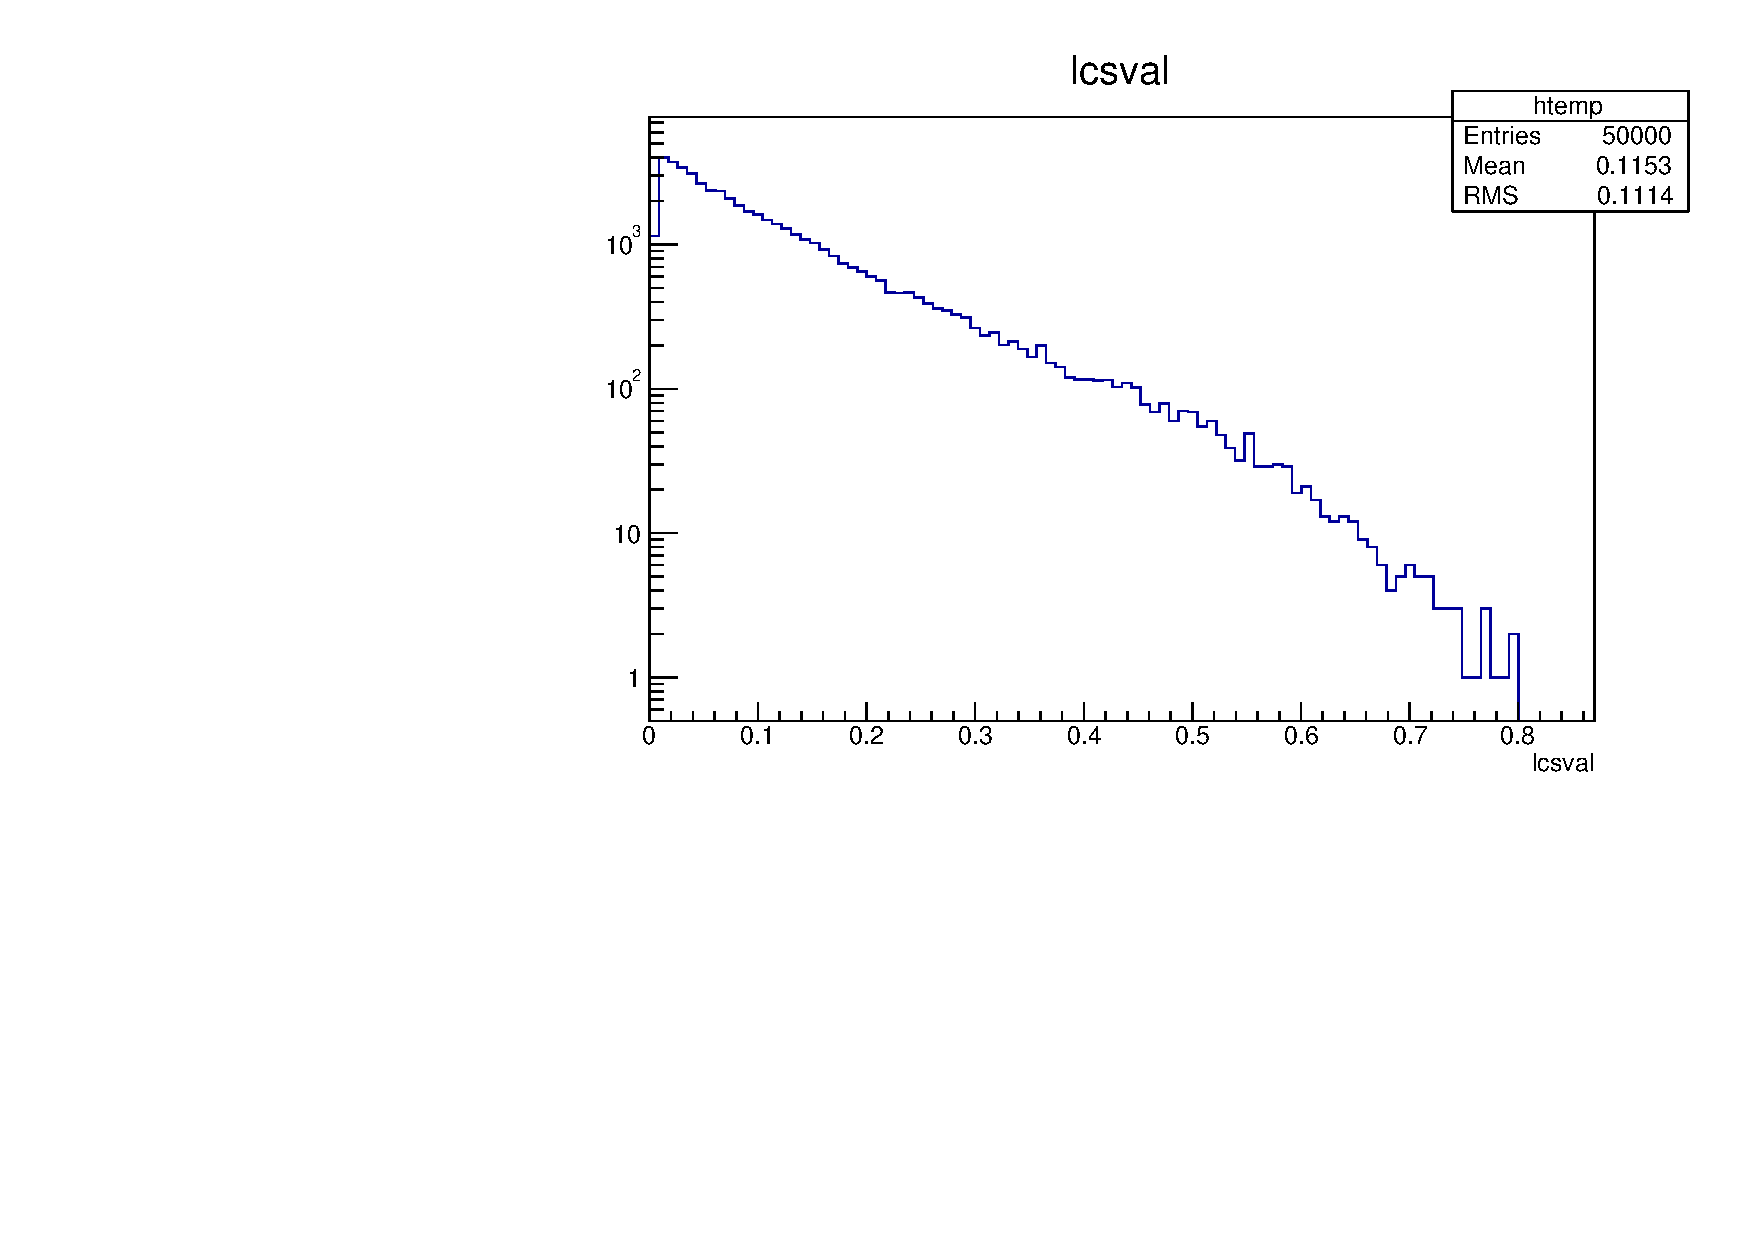
\includegraphics[width=6in,height=3in]{ldcs-value-KN.pdf} 
   \caption[]{Distribution of linearly polarized DCS for $\gamma p\rightarrow K^+\Lambda$}      \label{ldcs-value-KN}
   \end{center}
\end{figure}

  \end{itemize}

\item Unpolarized DCS table of $\pi^- p\rightarrow K^0\Lambda$ to calculate unpolarized DCS for the second step of channels 1 and 5 by isospin couplings and Clesch-Gordan coefficients. Table is built based on the Juelich model by D. Ronchen et al.
 \begin{itemize}
  \item Orignial and adjusted unpolarized DCS tables for $\pi^- p\rightarrow K^0\Lambda$: $W$: [1.626, 2.405] GeV; $\cos\theta_{cm}$: [-1, 1]
  \item Unpolarized DCS for $\pi^0 p\rightarrow K^+\Lambda$ and $\pi^+ n\rightarrow K^+\Lambda$: $\sigma_{\pi^- p\rightarrow K^0\Lambda}$ : $\sigma_{\pi^0 p\rightarrow K^+\Lambda}$ : $\sigma_{\pi^+ n\rightarrow K^+\Lambda}$ = 2 : 1 : 2
  \end{itemize}

\end{enumerate}

\section{Options}
\subsection{Options -R -M -h}
	-R [filename]: Output file with name [filename].root

	-M [\#]: Process  [\#] of events

	-h: Information for help

\subsection{Option -E}
	-E [expression]: Photon energy

         \begin{itemize}
	\item expression = x :          	Monoenergetic E = x GeV
	\item expression = x:y :       	Plain distribution from x to y GeV
	\item expression = mono:x :      	Monoenergetic as above
	\item expression = plain:x:y : 	Plain distribution as above
	\item expression = brems:x:y : 	Bremsstrahlung distribution 1/E
	\item expression = histo:[filename]:[hstname] :	Distribution according to 1 dimentional ROOT histogram [hstname] in [filename]
        \end{itemize}
         Whitespace is not allowed in the expression.

\subsection{Options -n -c}
	-n [\#]: [\#] channels are processed; Default: 9

	-c [***]: Processed channel number [***]; Must be followed after option `n'; Default: 123456789

	For example: -n 4 -c 2457 means 4 channels 2, 4, 5 and 7 are processed.

\subsection{Option -p}
	-p [argument]: Determine if implementing unpolarized(u) or circularly-polarized(c) or linearly-polarized(l) differential cross section for the first step. 

         \begin{itemize}
	 \item argument = ncs (default): Don't implement DCS
	 \item argument = ucs: Implement unpolarized DCS
          \item argument = ccs: Implement circularly polarized DCS
          \item argument = lcs: Implement linearly polarized DCS
          \end{itemize}

For all channels, ncs means not to implement differential cross section. For channels 2 and 8, ucs means implementing unpolarized DCS, ccs means implementing circularly polarized DCS and lcs means implementing linearly polarized DCS. For channels 1 and 5, ucs means implementing unpolarized DCS when argument is ucs or ccs since no circular ploarization observable tables can be applied for these two channels so that circularly polarized DCS can not be implemented, and lcs means implementing linearly polarized DCS. For channels 3, 4 and 9, unpolarized DCS is implemented when argument is ucs, ccs or lcs since no ploarization observable tables are applied for these three channels so that polarized DCS are not implemented. For channes 6 and 7, no corss section is implemented when argument is ncs, ucs, ccs or lcs since no unpolarized DCS tables can be applied for these two channels so that unpolarized and polarized DCS can not be implemented.

\subsection{Option -q}
	-q [argument]: Determine if implement unpolarized DCS for the second step of channels 1 and 5
         \begin{itemize}
	 \item argument = ncs (default): Don't implement DCS
	 \item argument = ocs: Implement unpolarized DCS using oringinal DCS table (longer running time)
	 \item argument = acs: Implement unpolarized DCS using adjusted DCS table (shorter running time)
          \end{itemize}
To shorten running time, the oringinal DCS table is adjusted so that kinematics are uniformly distributed in the table. The adjustment brings slight bias, so the option "-q" is offered to choose the originial table or the adjusted table. Figure~\ref{diff} shows the distribution of difference of calculated DCS with application of orignial and adjusted DCS tables. The figure suggests that the difference is slight.

\begin{figure}[H]
   \begin{center}
   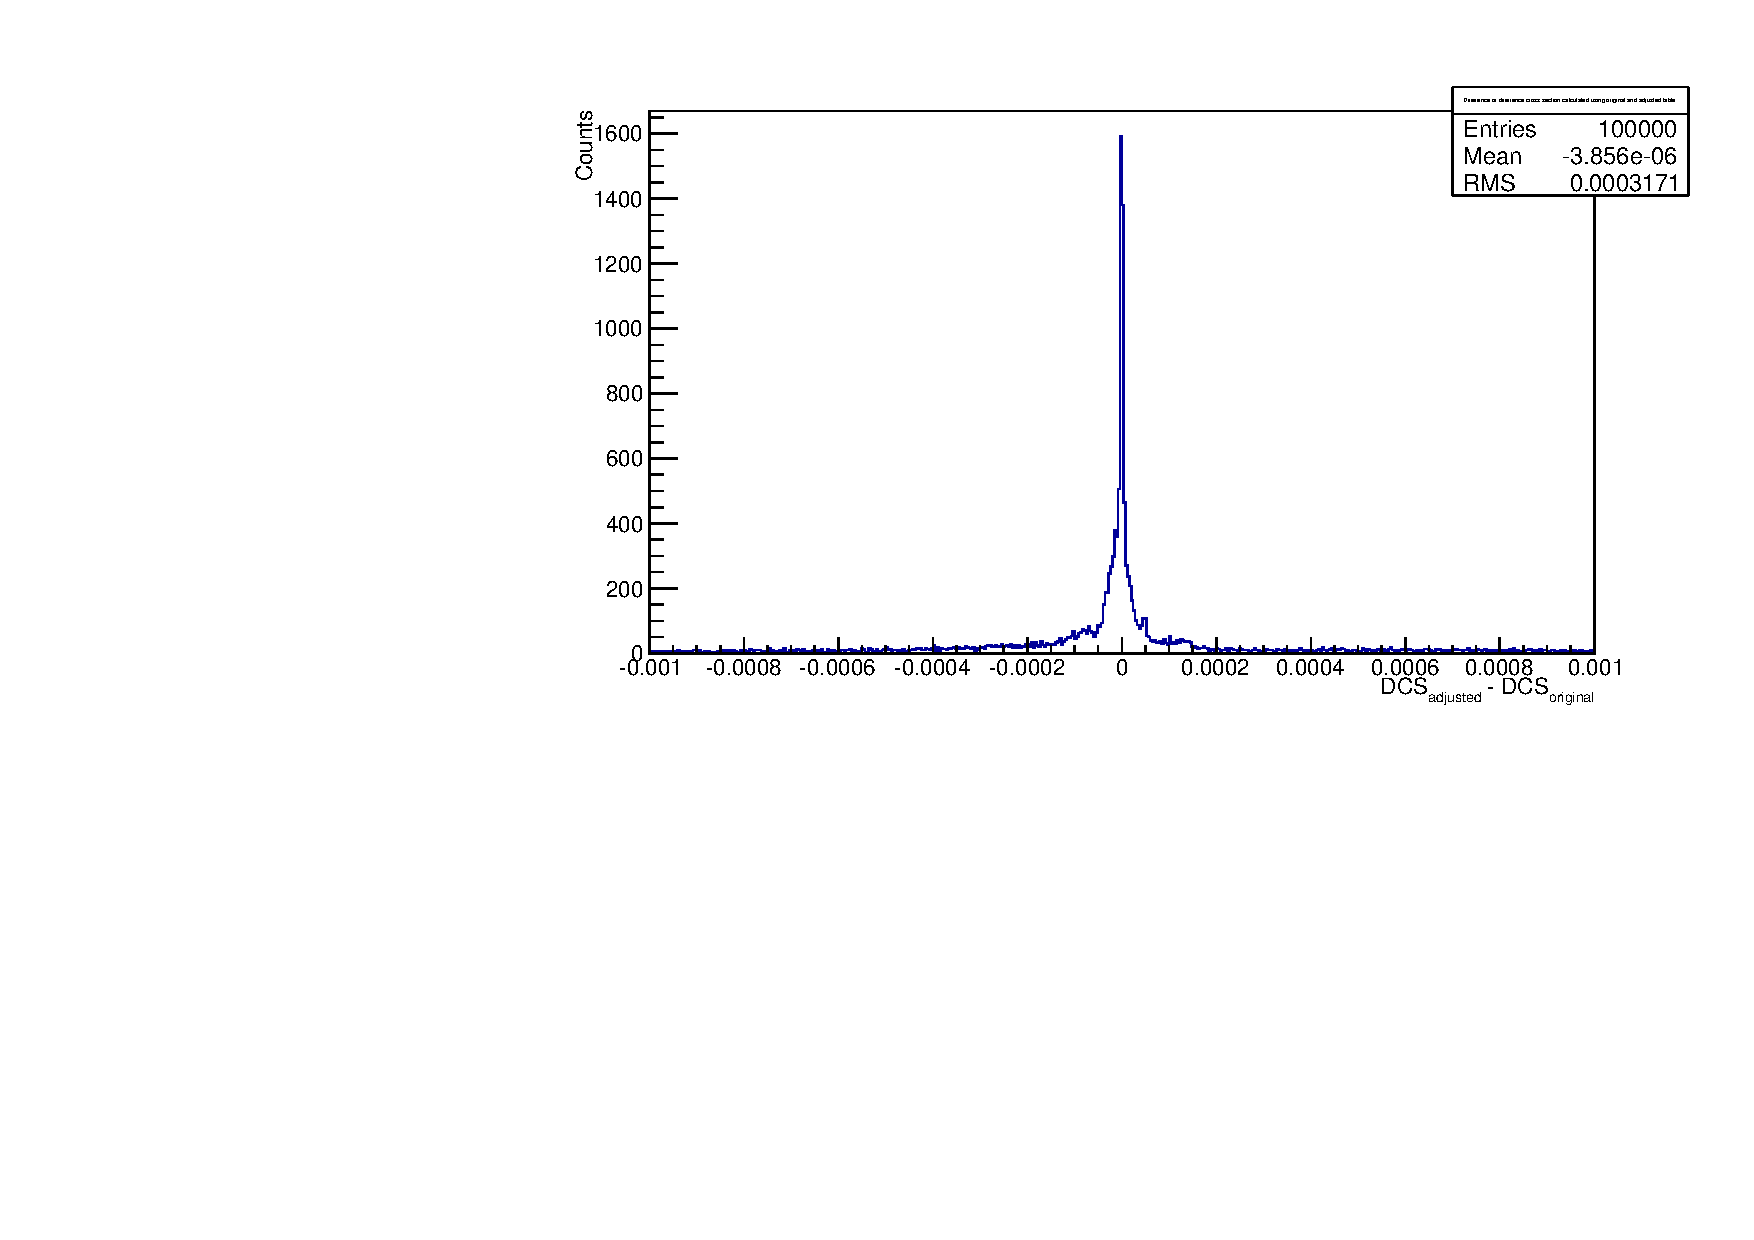
\includegraphics[width=6in,height=3.6in]{diff-ori-adj.pdf} 
   \caption[]{Difference of calculated DCS with application of original and adjusted DCS tables}      \label{diff}
   \end{center}
\end{figure}

\subsection{Option -s}
          -s [argument]: Determine if the maximum of RN3 is the same or different and if the other maximum of RN4L is the same or different
         \begin{itemize}
	 \item argument = diff (default): Different channels have different maximum values dependent of their own DCS table (shorter running time, unfair for channels)
	 \item argument = same: All channels have the same maximum value, which is maximum value of all tables (longer running time, fair for channels)
          \end{itemize}
RN3 is compared to unpolarized DCS of the first step to determine if an event is accpted or rejected. RN4L is compared to circularly polarized DCS of the first step to determine if an event is accepted or rejected. For fair comparison between channels, argument should be set as ``same", but the code-running time is much longer.

\section{Simple Introduction to Other Packages for Simulation}
The latest version of simulation packages is in /u/home/caot/simulation of JLab ifarm. Explanation for each package is as follows. 

\begin{itemize}
\item php: Codes for automatically downloading differential cross section from Said database and make differential cross section tables
\item KYcs: Isospin coupling technique is used to convert differential cross section from relevant channels to channels of our interests
\item PutInBOS: Convert root files generated from generator into BOSfile; Generate the reaction vertex and decay vertex
\item GSIM: Process events in simulated g13 environment
\item SkimGSIM: Preliminarily filter events
\item AutomateAll: A script file for executing the generator and a xml file for submitting jobs

\end{itemize}

\section{How to Run and Current Simulated Data Versions}
Users need to copy all packages from /u/home/caot/simulation of JLab ifarm and compile them, change the script file according to requirements of analysis, and change the xml file according to directories of input and output files.

Currently, 4 simulated data versions are saved in /lustre/expphy/volatile/clas/clasg13/caot/simulation. For each version, 1000 jobs were submitted and executed. Their generator commands are as follows:

\begin{itemize}
\item v1: ./generator -R generated\_\$\{RUNFILE\}.root -M 50000 -E 0.9:2.6 -p ccs -n 2 -c 28
\item v2: ./generator -R generated\_\$\{RUNFILE\}.root -M 50000 -E 0.9:2.6 -p lcs -q ocs -s same -n 5 -c 12358
\item v3: ./generator -R generated\_\$\{RUNFILE\}.root -M 50000 -E 0.9:2.6 -p ucs -q ncs -s same -n 7 -c 1234589
\item v4: ./generator -R generated\_\$\{RUNFILE\}.root -M 50000 -E 0.9:2.6
\end{itemize}

If implementing unpolarized or polarized DCS in the first step, it is better to exclude channels 6 and 7. Otherwise, events will be dominant by them since no unpolarized or polarized DCS is implemeted for these 2 channels. For different choises of options, running time of the generator may be different, but no effects for other packages.

\end{document}
